A base de dados em questão será usada para realização de tarefa de classificação multi-rótulo segundo o paradigma de aprendizado supervisionado. Nesta tarefa, exemplos de expressões faciais e seus respectivos rótulos serão fornecidos previamente aos modelos de Aprendizado de Máquina para escolha e ajuste de parâmetros e realização do treinamento. Posteriormente, expressões faciais ainda não vistas serão apresentadas e o objetivo será avaliar o desempenho do modelo na classificação destes exemplos, isto é, aferir a respectiva capacidade de generalização.

Obedecendo a uma partição do FER2013 previamente considerada em competições de Visão Computacional \cite{Kaggle:FER2013}, esta base de dados será dividida em $3$ partes, sendo: $80$\% dos exemplos para treinamento,  $10$\% dos exemplos para validação e $10$\% dos exemplos remanescentes para testes, a serem utilizados seguindo uma abordagem de \emph{holdout} de validação cruzada  \cite{Brink:MachineLearningLivro}.  Apenas os exemplos da partição de testes serão utilizados para obtenção das métricas de desempenho e comparação dos modelos. Conforme ilustra a Figura \ref{fig:particoes}, as partições preservam a distribuição de amostras por classe na base de dados original.

\begin{figure}[!htb]
	\centering
  	\caption{Distribuição das classes nas partições adotadas para o conjunto de dados.} \label{fig:particoes}
	\subfloat[Treinamento]{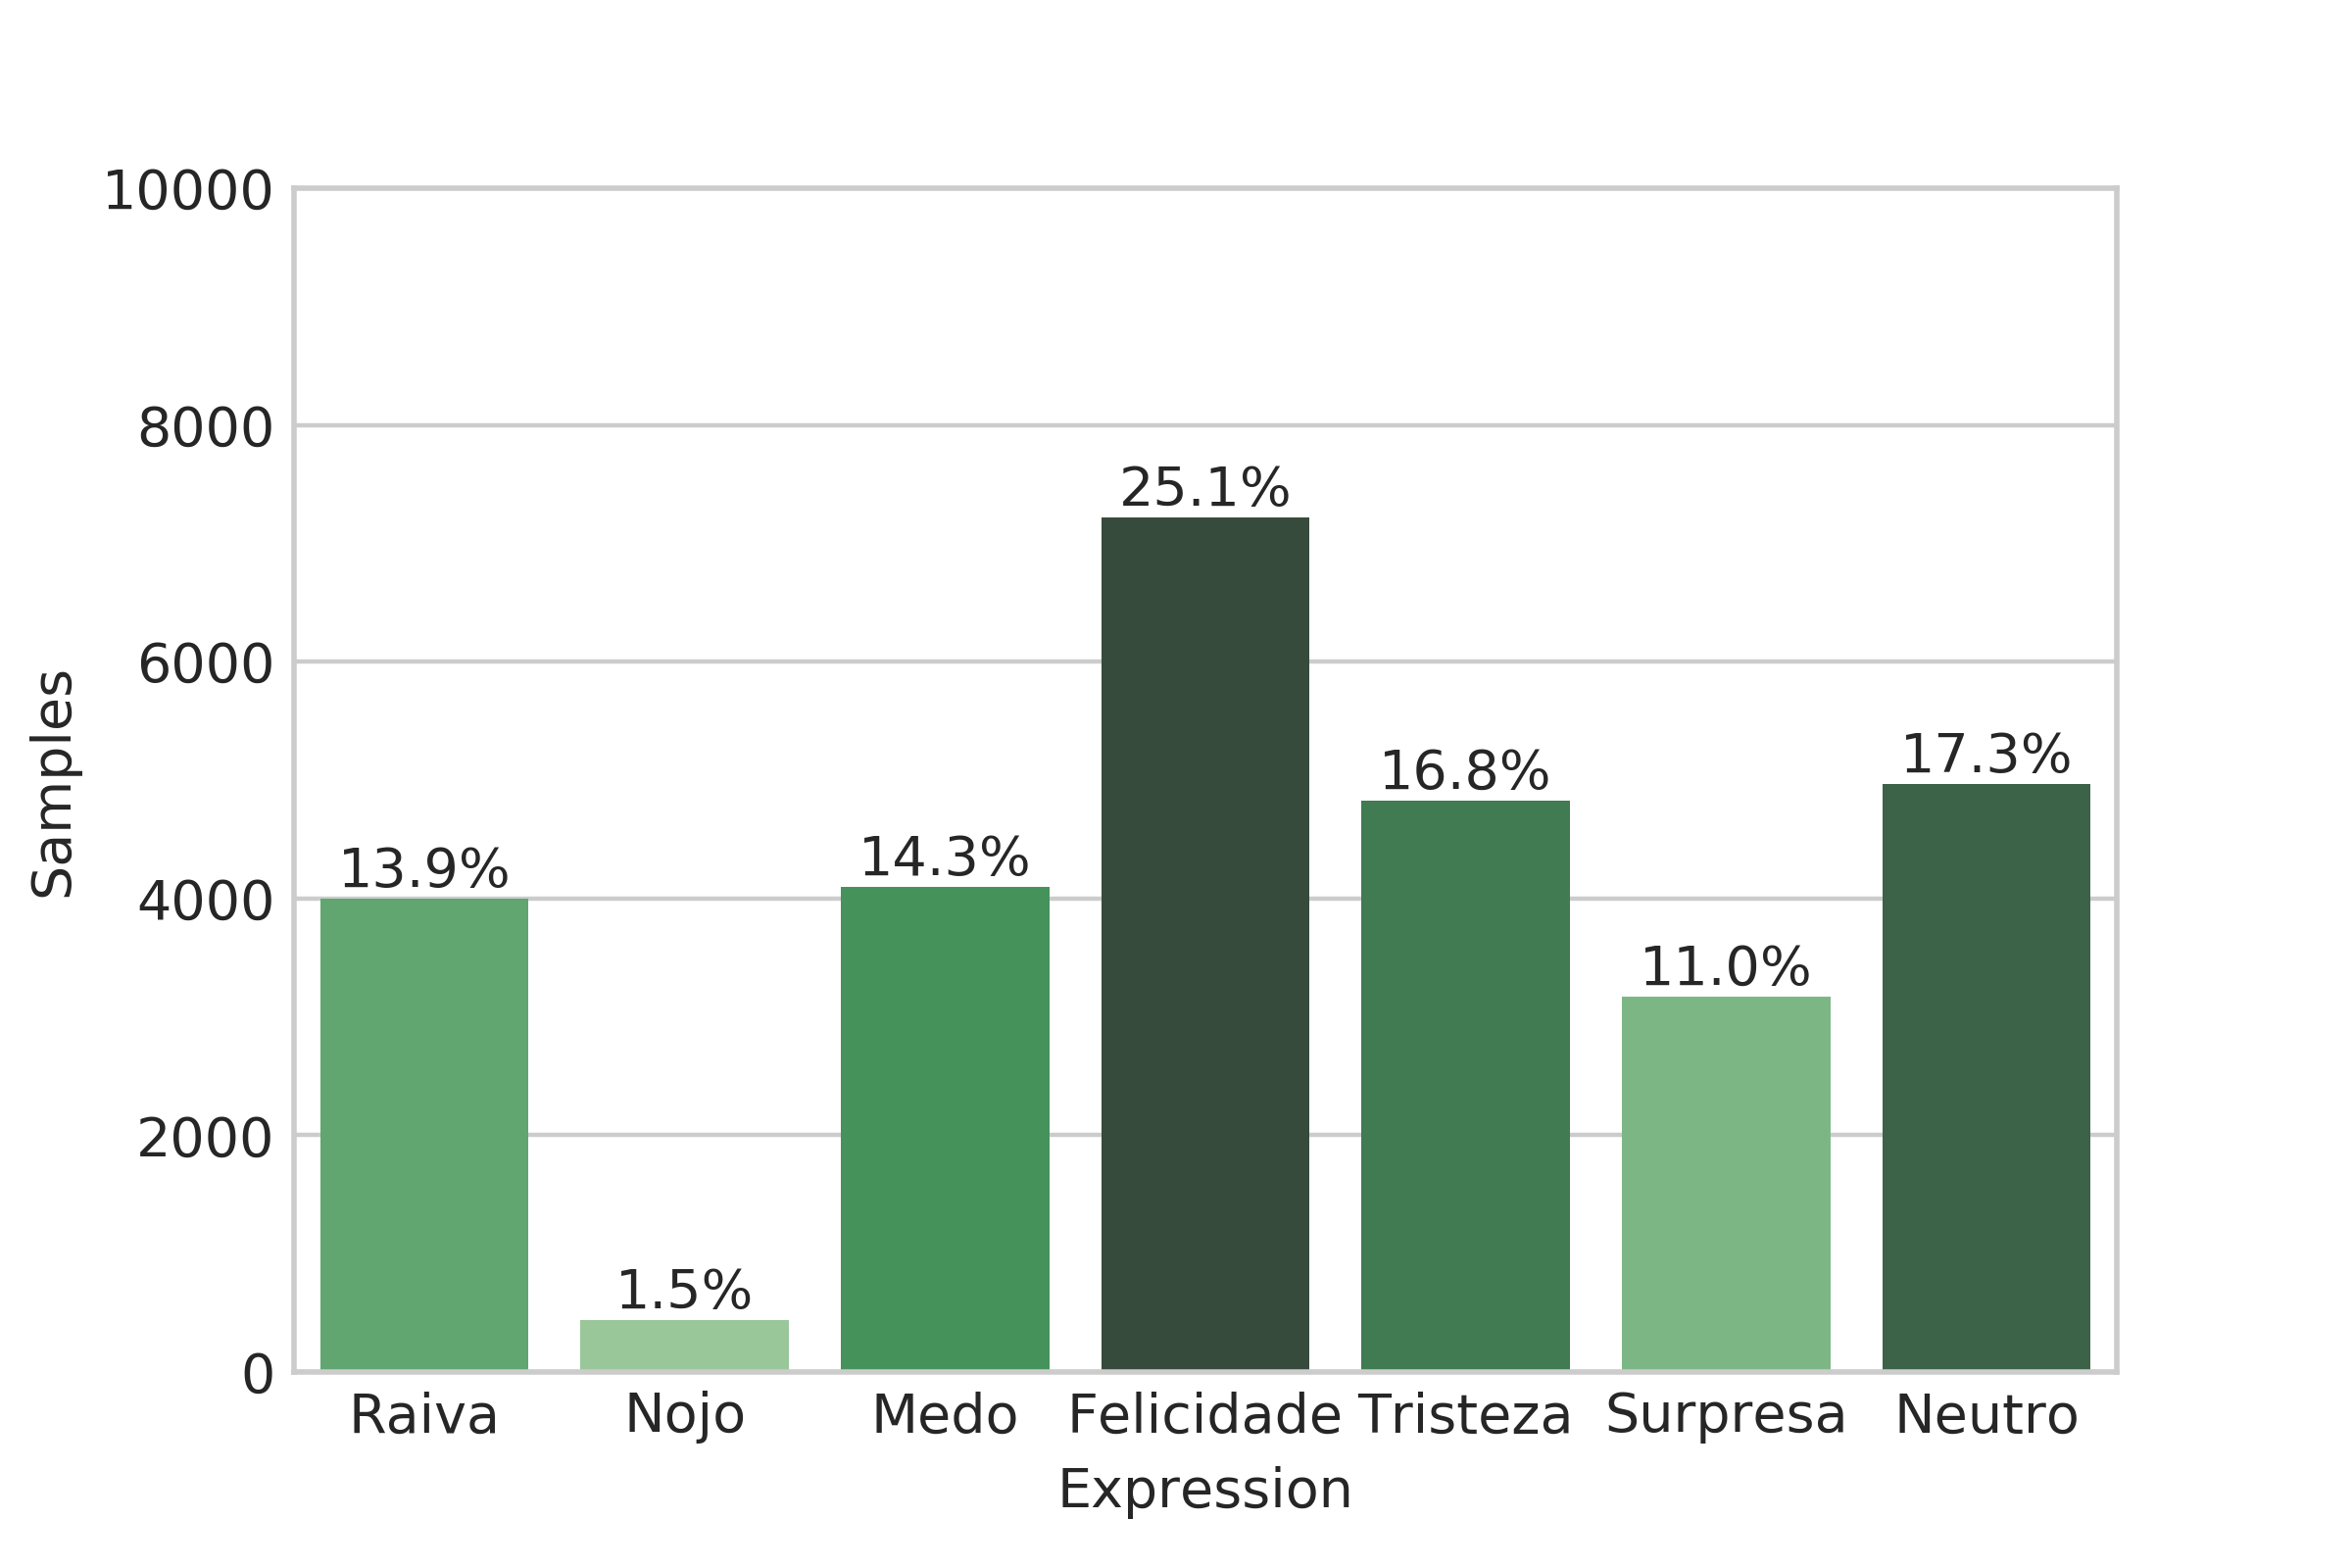
\includegraphics[width=0.33\linewidth]{images/expression_distribution_training.png}}
	\subfloat[Validação]{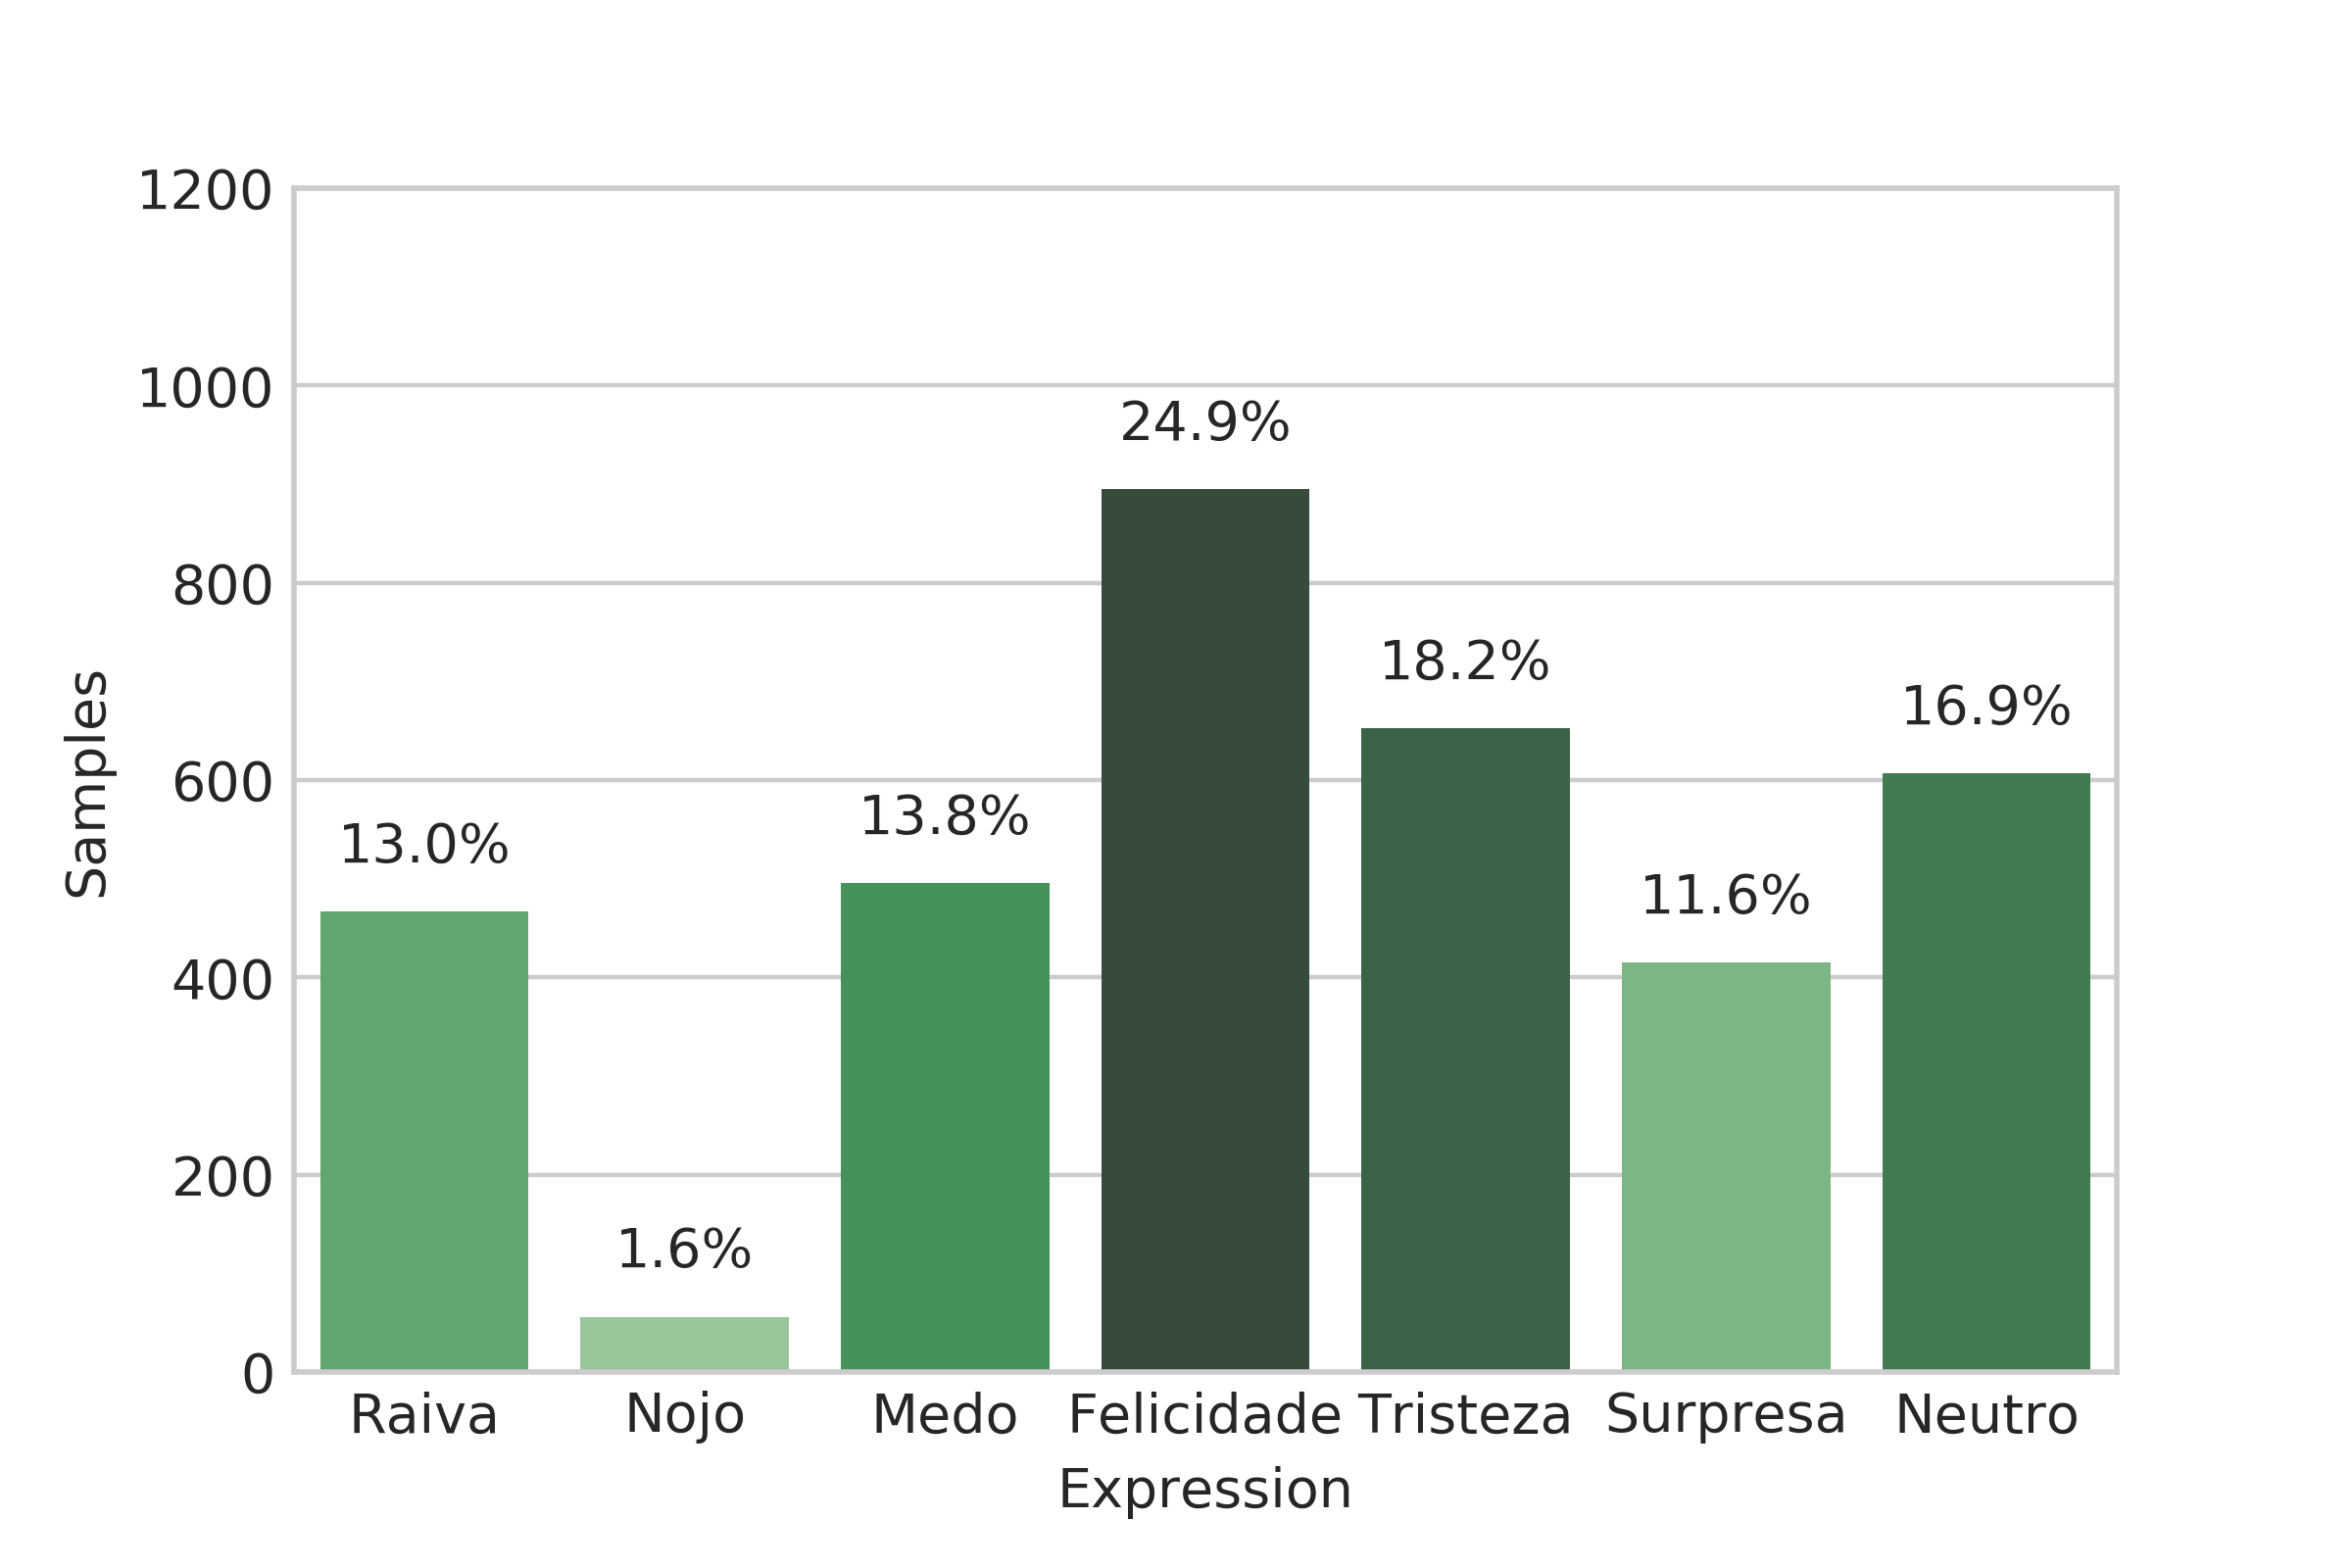
\includegraphics[width=0.33\linewidth]{images/expression_distribution_validation.png}}
	\subfloat[Teste]{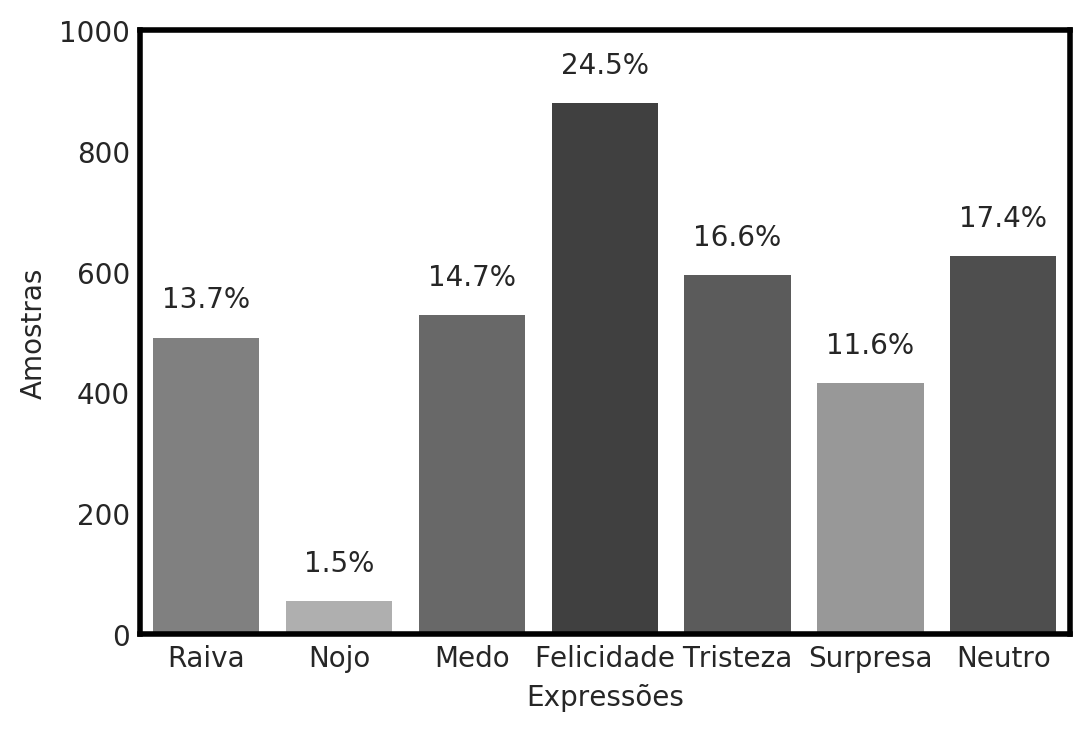
\includegraphics[width=0.33\linewidth]{images/expression_distribution_test.png}}
\end{figure}

Levando em conta os modelos de Aprendizagem de Máquina para a tarefa em questão, é essencial que um número razoável de exemplos esteja disponível para um ajuste apropriado dos parâmetros treináveis, pois com uma base de dados pequena estes ficam propensos a \textit{overfitting}, o que inibe a capacidade de generalização, em dados não vistos\cite{DBLP:journals/corr/abs-1708-06020}. Considerando esta necessidade prática, os exemplos da partição de treinamento passaram por um processo de pseudo-expansão do tipo \emph{data augmentation}, em que novas imagens foram geradas a partir das previamente existentes considerando transformações lineares de rotação, translação, escala e reflexão, colaborando para a posterior regularização dos modelos \cite{Chollet:Livro}, tornando-os invariantes aos tipos de operações realizadas\cite{DBLP:journals/corr/abs-1708-06020}. Que consistiram de rotação em módulo de até $10$\textordmasculine no sentido horário e anti-horário, translações de até $10$ pixels nas direções ortogonais, fator de escala em módulo de $4$ e reflexão em relação ao eixo das ordenadas. Ao final desta etapa, o conjunto de treinamento passou a conter $1.33\times10^{15}$ exemplos, um aumento de $3.70\times10^{10}$ vezes em relação ao seu tamanho original, mas preservando a distribuição de exemplos nas classes.

A métrica de desempenho adotada para comparação dos modelos na realização desta tarefa foi o Micro $F$-\emph{Score}. Embora a acurácia seja uma métrica mais popular, que descreve o percentual de acertos do modelo em relação ao total de previsões efetuadas, não fornece detalhes acerca dos acertos por classe. Para contornar esta dificuldade, o Micro $F$-\emph{Score} foi preferido, pois contempla a média harmônica entre precisão e revocação por classe ao passo que considera as diferentes frequências nas classes do problema \cite{Kubat:Livro}. Esta métrica é especialmente utilizada em problemas de classificação com classes desbalanceadas, ou seja, em situações análogas ao cenário considerado no escopo deste trabalho.

Dentre os modelos a serem avaliados, serão elencados como mais aptos para a tarefa de classificação proposta aqueles que maximizarem a métrica de desempenho Micro $F$-\emph{Score}  para os exemplos pertencentes à partição de testes.
